
%(BEGIN_QUESTION)
% Copyright 2014, Tony R. Kuphaldt, released under the Creative Commons Attribution License (v 1.0)
% This means you may do almost anything with this work of mine, so long as you give me proper credit

Anta at en Rosemount modell 3244MV (FOUNDATION Fieldbus) brukes som spenningssensor for en strekkmålebro, konfigurert for DC-mV inn og belastning i pounds force. Broen gir 1.5 mV per pund kraft:

$$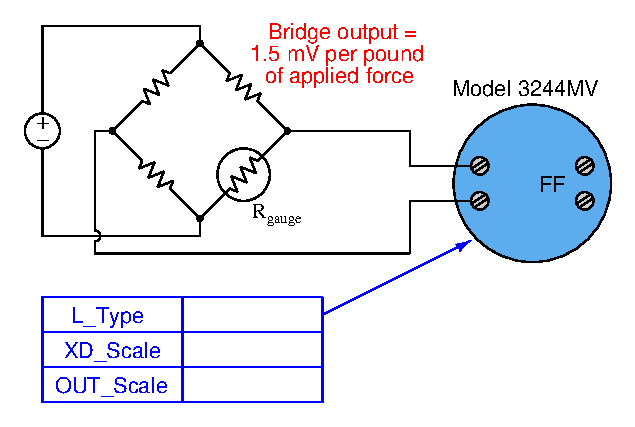
\includegraphics[width=15.5cm]{i00962x01.eps}$$

Bestem riktige {\tt XD\_Scale}, {\tt OUT\_Scale} og {\tt L\_Type} for område 0 til 35 pounds.

\underbar{file i00962}
%(END_QUESTION)





%(BEGIN_ANSWER)

{\tt L\_Type} = Indirect

\vskip 10pt

{\tt XD\_Scale} = 0 til 52.5 mV

\vskip 10pt

{\tt OUT\_Scale} = 0 til 35 pounds

%(END_ANSWER)





%(BEGIN_NOTES)

{\bf Denne oppgaven er ment kun for eksamen, ikke for arbeidsark!}.

%(END_NOTES)

